\documentclass[residuals.tex]{subfiles}
\begin{document}
\Large

\section{Regression Deletion Diagnostics}

This suite of functions can be used to compute some of the regression (leave-one-out deletion) diagnostics for linear and generalized linear models discussed in Belsley, Kuh and Welsch (1980), Cook and Weisberg (1982), etc.

\subsection*{Details}
\begin{itemize}
	\item The primary high-level function is \texttt{influence.measures} which produces a class "infl" object tabular display showing the DFBETAS for each model variable, DFFITS, covariance ratios, Cook's distances and the diagonal elements of the hat matrix. Cases which are influential with respect to any of these measures are marked with an asterisk. 
	
	\item The functions \texttt{dfbetas}, \texttt{dffits}, \texttt{covratio} and \texttt{cooks.distance} provide direct access to the corresponding diagnostic quantities. 
	
	\item Functions \texttt{rstandard} and \texttt{rstudent} give the standardized and Studentized residuals respectively. 
	
	\item (These functions re-normalize the residuals to have unit variance, using an overall and leave-one-out measure of the error variance respectively.) 
	
	\item Values for generalized linear models are approximations, as described in Williams (1987) (except that Cook's distances are scaled as F rather than as chi-square values). The approximations can be poor when some cases have large influence. 
	
	\item The optional i\texttt{nfl}, \texttt{res} and \texttt{sd} arguments are there to encourage the use of these direct access functions, in situations where, e.g., the underlying basic influence measures (from \texttt{lm.influence} or the generic influence) are already available. 
	
	\item Note that cases with \texttt{weights == 0} are dropped from all these functions, but that if a linear model has been fitted with \texttt{na.action = na.exclude}, suitable values are filled in for the cases excluded during fitting. 
	
	\item 
	The function \texttt{hat()} exists mainly for S (version 2) compatibility; we recommend using \texttt{hatvalues()} instead. 
\end{itemize}
 

\begin{framed}
	\begin{verbatim}
	Usage
	influence.measures(model)
	
	rstandard(model, ...)
	
	## S3 method for class 'lm'
	rstandard(model, infl = lm.influence(model, do.coef = FALSE),
	sd = sqrt(deviance(model)/df.residual(model)), ...)
	
	## S3 method for class 'glm'
	rstandard(model, infl = influence(model, do.coef = FALSE),
	type = c("deviance", "pearson"), ...)
	\end{verbatim}
\end{framed}

%==================================================== %
\begin{framed}
	\begin{verbatim}
	rstudent(model, ...)
	
	## S3 method for class 'lm'
	rstudent(model, infl = lm.influence(model, do.coef = FALSE),
	res = infl$wt.res, ...)
	
	## S3 method for class 'glm'
	rstudent(model, infl = influence(model, do.coef = FALSE), ...)
	
	dffits(model, infl = , res = )
	\end{verbatim}
\end{framed}
\newpage


\section{Standardized and Studentized Residuals}
The standardized residual is the residual divided by its standard deviation. 
 
Plot the standardized residual of the simple linear regression model of the data set faithful against the independent variable waiting.

We apply the lm function to a formula that describes the variable eruptions by the variable waiting, and save the linear regression model in a new variable eruption.lm. Then we compute the standardized residual with the rstandard function.

\begin{framed}
\begin{verbatim}
> eruption.lm = lm(eruptions ~ waiting, data=faithful) 
> eruption.stdres = rstandard(eruption.lm) 
\end{verbatim}
\end{framed}
We now plot the standardized residual against the observed values of the variable waiting.
\begin{framed}
\begin{verbatim}
> plot(faithful$waiting, eruption.stdres, 
+     ylab="Standardized Residuals", 
+     xlab="Waiting Time", 
+     main="Old Faithful Eruptions") 
> abline(0, 0)                  # the horizon
\end{verbatim}
\end{framed}


%--------------------------------------------------- % 
	\section{Leverage and Influence}
	\subsection{Influence}
	The influence of an observation can be thought of in terms of how much the predicted scores for other observations would differ if the observation in question were not included. 
	
%	Cook's D is a good measure of the influence of an observation and is proportional to the sum of the squared differences between predictions made with all observations in the analysis and predictions made leaving out the observation in question. If the predictions are the same with or without the observation in question, then the observation has no influence on the regression model. If the predictions differ greatly when the observation is not included in the analysis, then the observation is influential.
	
	
	\subsection{Influential Points}
	
	An influential point is an outlier that greatly affects the slope of the regression line. One way to test the influence of an outlier is to compute the regression equation with and without the outlier.
	
	This type of analysis is illustrated below. The scatter plots are identical, except that the plot on the right includes an outlier. The slope is flatter when the outlier is present (-3.32 vs. -4.10), so this outlier would be considered an influential point.
	
	\subsection{Without Outlier}
	
	% With Outlier
	
	\begin{itemize}
		\item Regression equation: $\hat{y} = 104.78 - 4.10x$
		\item Coefficient of determination: $R^2 = 0.94$ 
	\end{itemize}
	\begin{itemize}
		\item Regression equation: $\hat{y} = 97.51 - 3.32x$
		\item Coefficient of determination: $R^2 = 0.55$ 
	\end{itemize}
	
	The charts below compare regression statistics for another data set with and without an outlier. Here, the chart on the right has a single outlier, located at the high end of the X axis (where x = 24). As a result of that single outlier, the slope of the regression line changes greatly, from -2.5 to -1.6; so the outlier would be considered an influential point.
	
	% Without Outlier
	% With Outlier
	
	% Regression equation: ŷ = 92.54 - 2.5x
	% Slope: b0 = -2.5
	% Coefficient of determination: R2 = 0.46 
	
	% Regression equation: ŷ = 87.59 - 1.6x
	% Slope: b0 = -1.6
	% Coefficient of determination: R2 = 0.52 
	
	
	Sometimes, an influential point will cause the coefficient of determination to be bigger; sometimes, smaller. In the first example above, the coefficient of determination is smaller when the influential point is present (0.94 vs. 0.55). In the second example, it is bigger (0.46 vs. 0.52).
	
	If your data set includes an influential point, here are some things to consider.
	
	%--------------------------------------------------------------------------------------%
	
	\begin{itemize}
		\item An influential point may represent bad data, possibly the result of measurement error. If possible, check the validity of the data point.
		
		\item Compare the decisions that would be made based on regression equations defined with and without the influential point. If the equations lead to contrary decisions, use caution.
		
	\end{itemize}
	%Test Your Understanding of This Lesson
	%
	%In the context of regression analysis, which of the following statements are true?
	%
	% I. When the data set includes an influential point, the data set is nonlinear. 
	%II. Influential points always reduce the coefficient of determination. 
	%III. All outliers are influential data points. 
	%
	%(A) I only 
	%(B) II only 
	%(C) III only 
	%(D) All of the above 
	%(E) None of the above 
	%
	%Solution
	%
	%The correct answer is (E). Data sets with influential points can be linear or nonlinear. In this lesson, we went over an example in which an influential point increased the coefficient of determination. With respect to regression, outliers are influential only if they have a big effect on the regression equation. Sometimes, outliers do not have big effects. For example, when the data set is very large, a single outlier may not have a big effect on the regression equation.
	\subsection{Summary of Influence Statistics}
	\subsection{rstudent}
	The studentized residual RSTUDENT is estimated by $s(i)^2$ without the ith observation, not by $s^2$. For example,
	
	\[\mbox{RSTUDENT} = \frac{r_i}{s_{(i)} \sqrt{(1 - h_i)}} \]
	Observations with RSTUDENT larger than 2 in absolute value may need some attention.
	
	
	
	
	
	\begin{itemize}
		\item	\textbf{Studentized Residuals} – Residuals divided by their estimated standard errors (like t-statistics). Observations with values larger than 3 in absolute value are considered outliers.
		\item	\textbf{Leverage Values (Hat Diag)} – Measure of how far an observation is from the others in terms of the levels of the independent variables (not the dependent variable). Observations with values larger than $2(k+1)/n$ are considered to be potentially highly influential, where k is the number of predictors and n is the sample size.
		\item	\textbf{DFFITS} – Measure of how much an observation has effected its fitted value from the regression model. Values larger than $2\sqrt{(k+1)/n}$ in absolute value are considered highly influential. %Use standardized DFFITS in SPSS.
		\item	\textbf{DFBETAS} – Measure of how much an observation has effected the estimate of a regression coefficient (there is one DFBETA for each regression coefficient, including the intercept). Values larger than 2/sqrt(n) in absolute value are considered highly influential.
		\\
		The measure that measures how much impact each observation has on a particular predictor is DFBETAs The DFBETA for a predictor and for a particular observation is the difference between the regression coefficient calculated for all of the data and the regression coefficient calculated with the observation deleted, scaled by the standard error calculated with the observation deleted. 
		
		\item	\textbf{Cook’s D} – Measure of aggregate impact of each observation on the group of regression coefficients, as well as the group of fitted values. Values larger than 4/n are considered highly influential.
	\end{itemize}
	
	
\section{Other Measures of Influence}
The impact of an observation on a regression fitting can be determined by the difference between the estimated regression coefficient of a model with all observations and the estimated coefficient when the particular observation is deleted. The measure DFBETA is the studentized value of this difference.

Influence arises at two stages of the LME model. Firstly when $V$ is estimated by $\hat{V}$, and subsequent
estimations of the fixed and random regression coefficients $\beta$ and $u$, given $\hat{V}$.

\

\subsubsection{DFBETA}
A group of measures that measures how much impact each observation has on a particular predictor are the DFBETAs. The DFBETA for a predictor and for a particular observation is the difference between the regression coefficient calculated for all of the data and the regression coefficient calculated with the observation deleted,  scaled by the standard error calculated with the observation deleted.

%\subsubsection{DFBETA} %1.16.3
\begin{eqnarray}
DFBETA_{a} &=& \hat{\beta} - \hat{\beta}_{(a)} \\
&=& B(Y-Y_{\bar{a}}
\end{eqnarray}

For $k$ predictors in the mode, there ar $k+1$ dfbetas.

% Interpret


\subsubsection{DFFITS} %1.16.1
DFFITS is a statistical measured designed to a show how influential an observation is in a statistical model. It is closely related to the studentized residual.
\begin{displaymath} DFFITS = {\widehat{y_i} -
	\widehat{y_{i(k)}} \over s_{(k)} \sqrt{h_{ii}}} \end{displaymath}


\subsubsection{COVRATIO}
The COVRATIO statistic measures the change in 
the determinant of the covariance matrix of the estimates by deleting the ith observation:

\[ COVRATIO = \frac{det ( s^2_{(i)} (X_{(i)}'X_{(i)})^{-1} ) )}{ det ( s^2 (X'X)^{-1} ) }  \]
%Belsley, Kuh, and Welsch suggest that observations with

Observations with

\[|{COVRATIO} - 1| \ge \frac{3k}{n}\]
where k is the number of parameters in the model and n is the number of observations used to fit the model, are worth further investigation.

%\subsubsection{PRESS} %1.16.2
%The prediction residual sum of squares (PRESS) is an value associated with this calculation. When fitting linear models, PRESS can be used as a criterion for model selection, with smaller values indicating better model fits.
%\begin{equation}
%PRESS = \sum(y-y^{(k)})^2
%\end{equation}
%
%
%\begin{itemize}
%	\item $e_{-Q} = y_{Q} - x_{Q}\hat{\beta}^{-Q}$
%	\item $PRESS_{(U)} = y_{i} - x\hat{\beta}_{(U)}$
%\end{itemize}


%-------------------------------------------------------------- %
\newpage

\subsection{Influential Observations : DFBeta and DFBetas}
%% http://stats.stackexchange.com/questions/22161/how-to-read-cooks-distance-plots
%Cook's distance refers to how far, on average, predicted y-values will move if the observation in question is dropped from the data set. dfbeta refers to how much a parameter estimate changes if the observation in question is dropped from the data set. Note that with k covariates, there will be k+1 dfbetas (the intercept,$\beta_0$, and 1 $\beta$ for each covariate). Cook's distance is presumably more important to you if you are doing predictive modeling, whereas dfbeta is more important in explanatory modeling.



%-------------------------------------------------------------------------------------------%
\newpage
	
\section{Influential Points in Regression}
% - http://stattrek.com/regression/influential-points.aspx
 

%ometimes in regression analysis, a few data points have disproportionate effects on the slope of the regression equation. In this lesson, we describe how to identify those influential points.


\begin{figure}
\centering
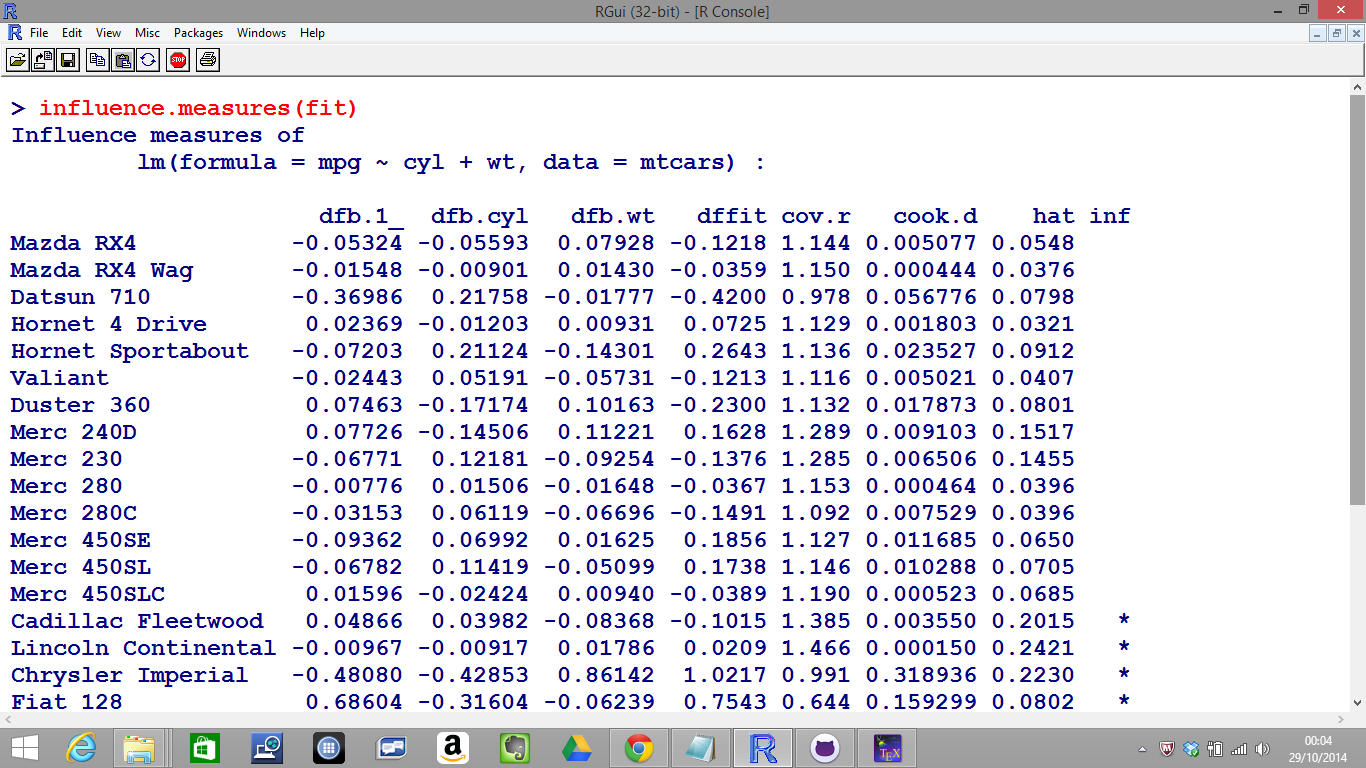
\includegraphics[width=1.1\linewidth]{Screenshot2}
\caption{}
\label{fig:Screenshot2}
\end{figure}


\begin{verbatim}
inflm.fit <- influence.measures(fit)
which(apply(inflm.fit$is.inf, 1, any))
\end{verbatim}
%-------------------------------------------------------------------------------------------%
\newpage


%==================================================== %
\begin{framed}
	\begin{verbatim}
	dfbeta(model, ...)
	## S3 method for class 'lm'
	dfbeta(model, infl = lm.influence(model, do.coef = TRUE), ...)
	
	dfbetas(model, ...)
	## S3 method for class 'lm'
	dfbetas(model, infl = lm.influence(model, do.coef = TRUE), ...)
	
	covratio(model, infl = lm.influence(model, do.coef = FALSE),
	res = weighted.residuals(model))
	\end{verbatim}
\end{framed}

%==================================================== %
\begin{framed}
	\begin{verbatim}
	cooks.distance(model, ...)
	## S3 method for class 'lm'
	cooks.distance(model, infl = lm.influence(model, do.coef = FALSE),
	res = weighted.residuals(model),
	sd = sqrt(deviance(model)/df.residual(model)),
	hat = infl$hat, ...)
	## S3 method for class 'glm'
	cooks.distance(model, infl = influence(model, do.coef = FALSE),
	res = infl$pear.res,
	dispersion = summary(model)$dispersion,
	hat = infl$hat, ...)
	\end{verbatim}
\end{framed}

%==================================================== %
\begin{framed}
	\begin{verbatim}
	hatvalues(model, ...)
	## S3 method for class 'lm'
	hatvalues(model, infl = lm.influence(model, do.coef = FALSE), ...)
	
	hat(x, intercept = TRUE)
	
	\end{verbatim}
\end{framed}
\begin{verbatim}
Arguments
model an R object, typically returned by lm or glm.

infl influence structure as returned by lm.influence or influence (the latter only for the glm method of rstudent and cooks.distance).

res (possibly weighted) residuals, with proper default.

sd standard deviation to use, see default.

dispersion dispersion (for glm objects) to use, see default.

hat hat values H[i,i], see default.

type type of residuals for glm method for rstandard.

x the X or design matrix.

intercept should an intercept column be prepended to x?

... further arguments passed to or from other methods.

\end{verbatim}

%========================================================================================== %
\newpage




\end{document}